Findings from previous chapters about privacy, routines and context integration indicate that the field of Ambient Information Systems is highly relevant in designing interactive domestic technology for personal financial management. This is because these systems focus on blending into the environment and presenting information in subtle ways that can potentially only be understood by the owners of the systems. In this regard we find that Informative Art is a particularly good source of inspiration. Furthermore, we believe that knowledge about Personal Informatics (Quantified Self) and self-reflection is valuable to understand how we may better support economic awareness and as it is highly related to data representations, which is one of the discovered themes in the previous chapter.

\section{Ambient Information Systems}
Since the foundation of Ubiquitous Computing, thoughts of calmer and more environmentally appropriate and integrated ways of conveying information have appealed to researchers and designers. This is largely contributed to Weiser’s visions about “calm computing” \cite{weiser1997coming} where he describes technology that is able to shift to the user’s attention when needed and otherwise stay calmly at the user’s periphery. Different directions of research that built on Weiser’s visions goes by various names such as “peripheral displays”, “ambient displays” and “notification systems”. These have all been brought together by Pousman and Stasko who propose the term Ambient Information Systems (AIS) for this overall body of work \cite{pousman2006taxonomy}. To understand the differences between these sub-domains one has to understand the underlying design motivations that informed them. The category of peripheral displays is the broadest and contains systems that may appear in the environment, on a secondary or even primary computer display. Ambient displays are a subset of peripheral displays, that are highly motivated by aesthetic goals and aspire to convey a small number of information elements. Notification systems are motivated by divided attention situations, where work tasks can be either primary or secondary in their attentional requirements. In the case of secondary work tasks these systems can be defined as peripheral.
AIS as a direction of study are defined by Pousman and Stasko to have specific behavioral characteristics \cite{pousman2006taxonomy}:

\vspace{12pt}
\begin{itemize}
	\item Present information that is important but not critical.
	\item Able to move from the periphery to the focus of attention and back again
	\item Focus on tangibility and representations in the environment
	\item Undistracting subtle changes that reflect updates in information
	\item Aesthetically pleasing and environmentally appropriate
\end{itemize}
\vspace{12pt}

In designing AIS decisions must be made regarding how much information to display, the specific aspects or elements to depict and how to display it. In the context of these decisions Pousman and Stasko present a taxonomy consisting of four design dimensions that constitute the space of AIS \cite{pousman2006taxonomy}: \emph{information capacity}, \emph{notification level}, \emph{representational fidelity} and \emph{aesthetic emphasis}. This taxonomy is essential to our work as it has informed the design choices in our exploration of the design space. For this reason the four design dimensions of the taxonomy are explained in relatively high detail in the following sections.

\subsection{Information Capacity}
Information capacity is described as the number of discrete information sources that a system is able to represent. Some system are only capable of displaying a single piece of information whereas others are able to display numerous or arbitrarily many. Pousman and Stasko call these pieces of discrete information “nuggets”. They argue that there is a design trade-off between space and time when considering information capacity. The information capacity of a display can be increased by expanding the space for information or by making the display transition through several views over a period of time. A system that uses multiple views or loops through views is naturally rated as having high information capacity since there, theoretically, is no limit to the number of information nuggets. Systems that have low ratings are typically physical displays that are purposely built to convey specific information using few information nuggets.

\subsection{Notification Level}
The notification level describes the degree to which system notifications are designed to interrupt the user, which directly relates to the relative importance of the information being conveyed -- the importance of the information should reflect the attention it demands. Pousman and Stasko base this design dimension on the work of Matthews et al. \cite{matthews2004toolkit} who define five notification levels: \emph{ignore}, \emph{change blind}, \emph{make aware}, \emph{interrupt} and \emph{demand attention}. These notification levels are grounded in attention literature that categorizes human attention into three types: \emph{inattention}, \emph{divided attention} and \emph{focused attention}. Inattention means that objects do not call for conscious awareness but may still affect behavior. In divided attention, stimuli is perceived such that attention is distributed over several objects and in focused attention all attention is focused on a single stimulus. Change blind represents information of minimal importance that is displayed in a way to not affect conscious awareness, corresponding to inattention. Make aware portrays information of some importance that calls for some attention, corresponding to divided attention. Interrupt and demand attention represent important information that should capture focused attention, meaning that the user is distracted from his current activity to attend to the system. Furthermore, demand attention also requires the user to perform some kind of action to stop the alerting. Notification level can be considered as the ambience of the system; systems that focus on unobtrusive make aware and change blind notifications are at the core of the ambient information system design space, while systems that use the interrupt or demand attention levels are further from the core.

\subsection{Representational Fidelity}
Representational fidelity describes an ambient information system’s display components and how data is encoded into words, sound, patterns and pictures. It can be thought of as the level of abstraction, where some systems portray the information being monitored very directly while others provide purely abstract representations. Pousman and Stasko describe representational fidelity using the theory of Semiotics, which is the study of signs and their meanings. A semiotic sign consists of three core parts. The object is called the \emph{signified} and is the physical thing or idea that the sign represents. The \emph{signifier} is the representation of the object (the signified) and \emph{sense} is the understanding that one arrives at from observing or experiencing the signified or the signifier. Semiotic signs can be \emph{symbolic}, \emph{iconic} or \emph{indexical} which can be directly translated to different levels of representational fidelity (from low to high respectively). Symbolic signs correspond to low fidelity because they are abstract and require some kind of rule-following convention to understand e.g. numbers, language characters and abstract visual representations. Iconic signs have a medium representational fidelity as they contain some transparency regarding the signified object e.g. metaphors and drawings. Lastly, indexical signs have a high representational fidelity as they are directly linked to the signified object, for example photographs.

\subsection{Aesthetic Emphasis}
The last design dimension is aesthetic emphasis which focuses on the importance of the aesthetics of the system. Judging aesthetics is fundamentally a subjective endeavour which makes it unfit to objectively decide a system’s aesthetic emphasis, therefore it is instead judged on the significance given to the aesthetics by the designers. High aesthetic emphasis is common when designing for visually pleasing displays intended to leverage the work of artists or for physical AIS that are often sculptural in their designs. Systems that are considered to be of medium aesthetic emphasis are those that are not intended to be art objects but are still explicitly intended to be seen as calm and visually pleasing systems. Lastly, systems that prioritise information conveyance over aesthetics are considered to have low aesthetic emphasis but they can still be calm and environmentally appropriate even though there is no explicit focus on aesthetic aspects.

\section{Informative Art}
In 2000 Redström et al. \cite{redstrom2000informative} presented the idea of Informative Art. They denote Informative Art as a combination of artwork and various objects/surfaces through which digital information can be presented. It is described as a type of slow technology, i.e. it promotes moments of attention and reflection, and aims to \emph{“augment a traditional notion of art objects, turning the given type of design surface into an abstract information display”} \cite[p.~104]{redstrom2000informative}. By embedding small pieces of digital information into structures or compositions Informative Art strives to give invisible information, such as website traffic or e-mail activity, form through digital artwork. Since Informative Art is designed to occupy architectural space, very much like paintings and posters, and is viewed as an integrated part of the physical environment a high focus on visual aesthetics is needed. This focus on aesthetics can be found in Pousman and Stasko’s \cite{pousman2006taxonomy} article where they describe Informative Art, using their taxonomy, as having a relatively low information capacity, a medium notification level, a low to medium representational fidelity and a high emphasis on aesthetics. Also, as prescribed by the notion of AIS, Informative Art is a type of technology that is designed to support peripheral information. In relation to their notation about technological artwork Redström et al. uses a term called Amplified Reality. They describe it as \emph{“the enhancement of expression or functionality of artefacts using technology”} \cite[p.~105]{pousman2006taxonomy} where the central point is on the physical presence of artifacts and not on some superimposed digital information laid on top of the “real world”. In other words, it is about enriching the expression of the real world rather than enhancing the impression of it.

\begin{figure}[h]
	\centering
	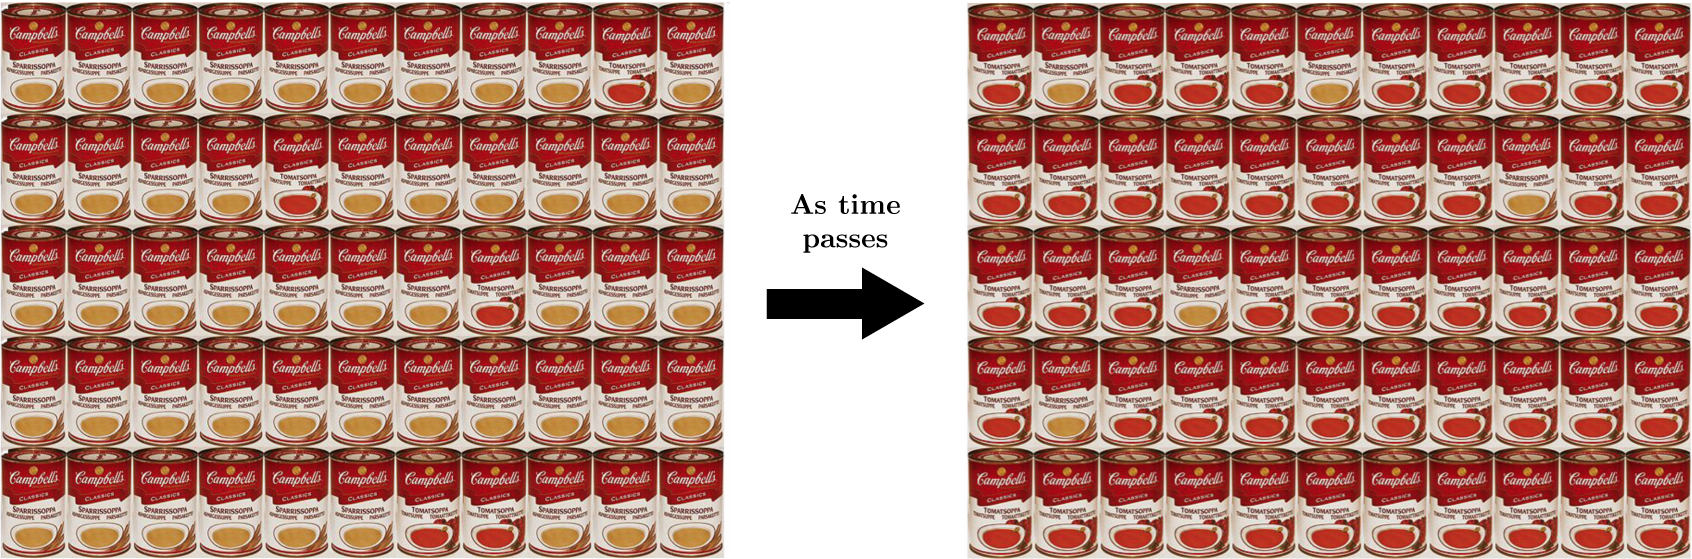
\includegraphics[width=\textwidth]{soup-clock}
	\caption{A countdown timer inspired by Andy Warhol's paintings. Courtesy to \cite{holmquist2003informative}}
	\label{fig:soup-clock}
\end{figure}

In 2002 Holmquist and Skog \cite{holmquist2003informative} presented an Informative Art installation which was exhibit at the SIGGRAPH 2001 Emerging Technologies. Using a set of projectors, a laptop running various Java applications and white textile they depicted different types of data through artwork. One of the more interesting pieces of art was Soup Clock; a simple egg timer (see figure~\ref{fig:soup-clock}. Through a repeated pattern of asparagus (yellow) and tomato (red) soup cans the passing of time was illustrated -- in the beginning of time the graphic only shows yellow soup cans and as time passes a yellow soup can gets substituted with a red soup can. A decade later Fan et al. \cite{fan2012spark} attempted to use Informative Art to visualize personal activity using data from Fitbit (a personal activity tracker). Through a tablet, placed in a common space in the home, the participants could select between different types of abstract data representations (see figure~\ref{fig:spark})that pictured step count and intensity. When interacting with the system the participants could obtain more details like time for the exercise and exact step count. By the end of the paper Fan et al. presents three elements that seemed to motivate their participants, namely the use of color to indicate activity intensity, movement in the graphic and filling up the screen with graphic. All these visual rewards might also be applicable to our project.

\begin{figure}[h]
	\centering
	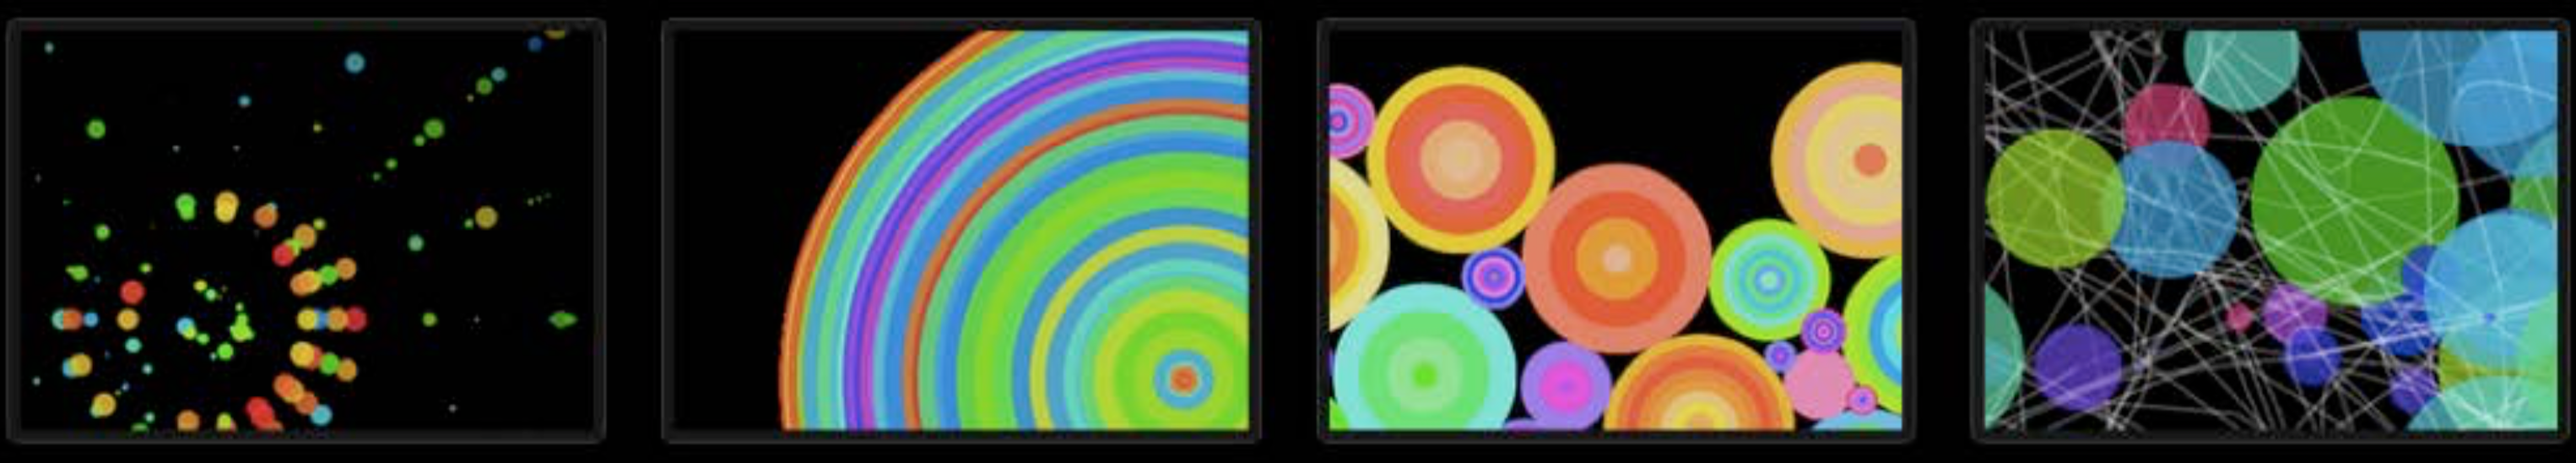
\includegraphics[width=\textwidth]{spark}
	\caption{Different data representations for Spark. Courtesy to \cite{fan2012spark}}
	\label{fig:spark}
\end{figure}

For our work we find the technical implementation for Soup Clock very interesting as it can be used to augment an existing architectural space and thereby creates a sense of domestic “belonging”. Even though Fan et al.’s solution does not have a high emphasis on visual aesthetic -- at least we do not view tablets as visually pleasing -- there is something to be learned from their work on personal informatics and data representation. The work of Informative Art resonates well with our findings from the workshop, thus we have used it as a source of inspiration for our project.

\section{Personal Reflection}
As technology matures and becomes more ubiquitous the ease of gathering personal information grows. According to Li et al. many tools have been developed to utilize this data in order to support self-reflection, yet these tools do not seem to meet the users’ needs \cite{li2011understanding}. In previous work Li et al. described these tools using the term Personal Informatics systems which is \emph{“systems that help people collect personally relevant information for the purpose of self-reflection and gaining self-knowledge”} \cite[p.~558]{li2010stage}. To achieve a better understanding of the problem space for Personal Informatics, Li et al. conducted a study where they set out to investigate what kinds of questions people usually asked about their data and why \cite{li2011understanding}. They identified the following six categories of questions: Status, History, Goal, Discrepancies, Context and Factors. Status refers to act of glancing at some data to determine whether or not a goal (e.g. drink two litres of water each day) has been met and if an action is needed to do so. History can be described as looking for trends and patterns in long-term data in order to get a sense of the overall progress (e.g. being on the path to achieve a goal or not). The third category, Goal, can be formulated in various levels of abstraction, however Li et al. use two types of goals, namely principle goal and program goal. Principle goals are related to achieving an ideal, for instance to become more productive, whereas the program-level goal represents a specific task which needs to be performed in order to achieve the principle goal, e.g. spend less time on social media. Discrepancies is somewhat intertwined with the Status category as it denotes the action of looking at the current status and then compare it with the goal, e.g. what is the difference between the goal and the current status. The last two categories, Context and Factors, are related to events or elements that in some degree influence the progress towards the goal. For instance, is food going to have an impact on the productivity.

In the pursuit of self-knowledge Li et al. found two phases to be prevalent. The first phase is the Maintenance phase where users have identified their goals and know which factors that have an affect on their progress. Users in this phase will often ask questions within the categories of Status and Discrepancy. The second phase is called Discovery and is characterized by a lack of goal and often users have failed to identify the factors that have an impact on their behaviour. People in this phase are asking questions regarding the History, Goals, Context and Factors. Depending on the phase different strategies can be applied to support the users, for example in the Maintenance phase it can be a good idea to alert the users when they are not meeting their goal.

As we are trying to develop an artifact for economic awareness an understanding of Personal Informatics is paramount. We aim to make use of the basic ideas presented in this section as we believe this will benefit our work greatly.
